\documentclass[11pt,a4paper]{article}
\usepackage{graphicx}
\usepackage{tcolorbox}
\usepackage{xcolor}
\usepackage{geometry}
\usepackage{tikz}
\usetikzlibrary{shapes.geometric, arrows}
\geometry{margin=0.8in}

% Define colors
\definecolor{mlblue}{RGB}{31, 119, 180}
\definecolor{mlorange}{RGB}{255, 127, 14}
\definecolor{mlgreen}{RGB}{44, 160, 44}
\definecolor{mlred}{RGB}{214, 39, 40}
\definecolor{mlpurple}{RGB}{148, 103, 189}
\definecolor{mlyellow}{RGB}{241, 196, 15}

\title{\Large\textbf{Discovery 3: Innovation Safari}\\
\vspace{0.3em}
\normalsize The Diamond Journey}
\date{}

\begin{document}
\maketitle
\vspace{-2em}

\section*{The Innovation Diamond}

\begin{center}
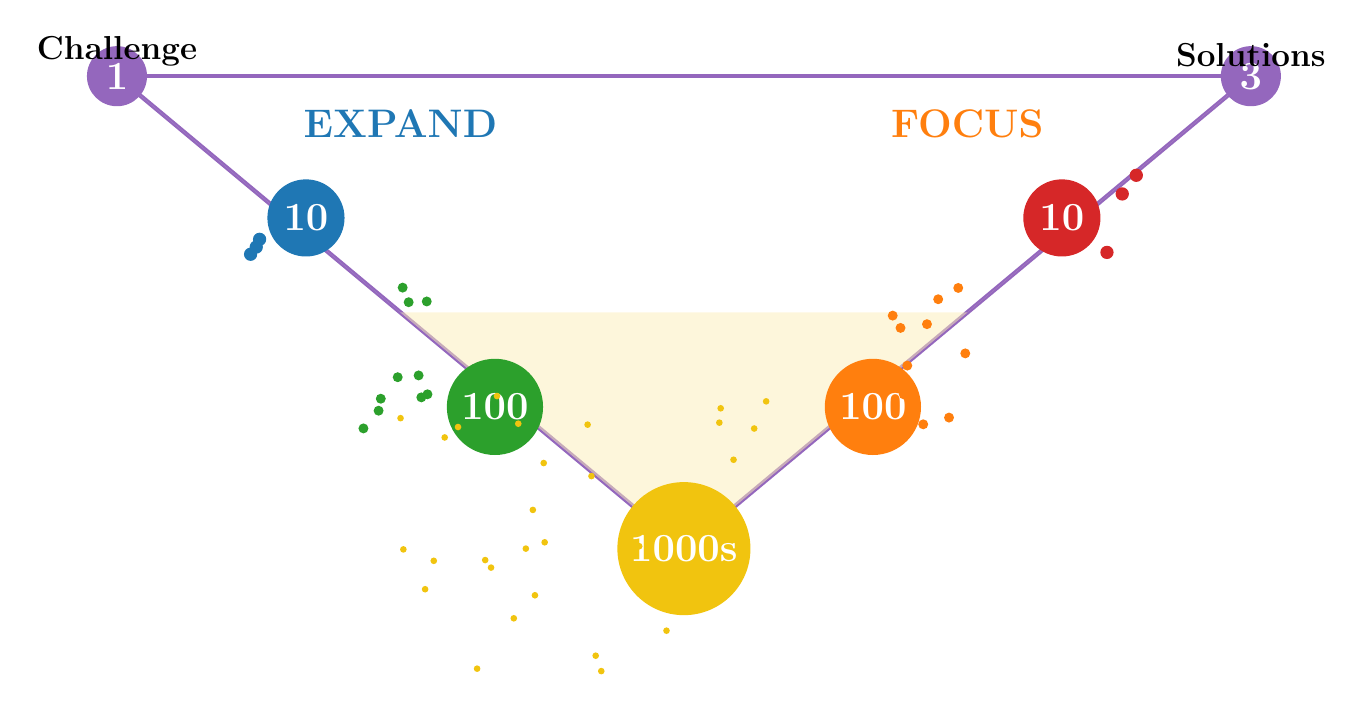
\begin{tikzpicture}[scale=1.2]
% Diamond shape outline
\draw[ultra thick, mlpurple] (0,5) -- (3,2.5) -- (6,0) -- (9,2.5) -- (12,5);
\draw[ultra thick, mlpurple] (0,5) -- (12,5);

% Fill regions with different colors
\fill[mlblue!20, opacity=0.5] (0,5) -- (3,2.5) -- (6,0) -- (3,2.5) -- cycle;
\fill[mlyellow!30, opacity=0.5] (3,2.5) -- (6,0) -- (9,2.5) -- cycle;
\fill[mlorange!20, opacity=0.5] (6,0) -- (9,2.5) -- (12,5) -- (9,2.5) -- cycle;

% Numbers at key points
\node[circle, fill=mlpurple, text=white, font=\Large\bfseries] at (0,5) {1};
\node[circle, fill=mlblue, text=white, font=\Large\bfseries] at (2,3.5) {10};
\node[circle, fill=mlgreen, text=white, font=\Large\bfseries] at (4,1.5) {100};
\node[circle, fill=mlyellow, text=white, font=\Large\bfseries] at (6,0) {1000s};
\node[circle, fill=mlorange, text=white, font=\Large\bfseries] at (8,1.5) {100};
\node[circle, fill=mlred, text=white, font=\Large\bfseries] at (10,3.5) {10};
\node[circle, fill=mlpurple, text=white, font=\Large\bfseries] at (12,5) {3};

% Phase labels
\node[font=\Large\bfseries, mlblue] at (3,4.5) {EXPAND};
\node[font=\Large\bfseries, mlorange] at (9,4.5) {FOCUS};

% Start and end labels
\node[above, font=\large\bfseries] at (0,5) {Challenge};
\node[above, font=\large\bfseries] at (12,5) {Solutions};

% Visual representation of ideas
\foreach \i in {1,...,3} {
    \pgfmathsetmacro{\x}{1.5 + rand*0.3}
    \pgfmathsetmacro{\y}{3.5 + rand*0.5}
    \fill[mlblue] (\x,\y) circle (2pt);
}
\foreach \i in {1,...,10} {
    \pgfmathsetmacro{\x}{3 + rand*0.5}
    \pgfmathsetmacro{\y}{2 + rand*0.8}
    \fill[mlgreen] (\x,\y) circle (1.5pt);
}
\foreach \i in {1,...,30} {
    \pgfmathsetmacro{\x}{5 + rand*2}
    \pgfmathsetmacro{\y}{0.2 + rand*1.5}
    \fill[mlyellow] (\x,\y) circle (1pt);
}
\foreach \i in {1,...,10} {
    \pgfmathsetmacro{\x}{8.5 + rand*0.5}
    \pgfmathsetmacro{\y}{2 + rand*0.8}
    \fill[mlorange] (\x,\y) circle (1.5pt);
}
\foreach \i in {1,...,3} {
    \pgfmathsetmacro{\x}{10.5 + rand*0.3}
    \pgfmathsetmacro{\y}{3.5 + rand*0.5}
    \fill[mlred] (\x,\y) circle (2pt);
}
\end{tikzpicture}
\end{center}

\vspace{1em}

\begin{tcolorbox}[colback=mlpurple!10, colframe=mlpurple!50]
\centering\Large
\textbf{Your Challenge: ``Make campus more sustainable''}
\end{tcolorbox}

\vspace{2em}

\section*{Phase 1: Expand (You have 3 minutes)}

\begin{center}
\Large
Write/draw as many ideas as you can. Don't think, just create!

\vspace{1em}

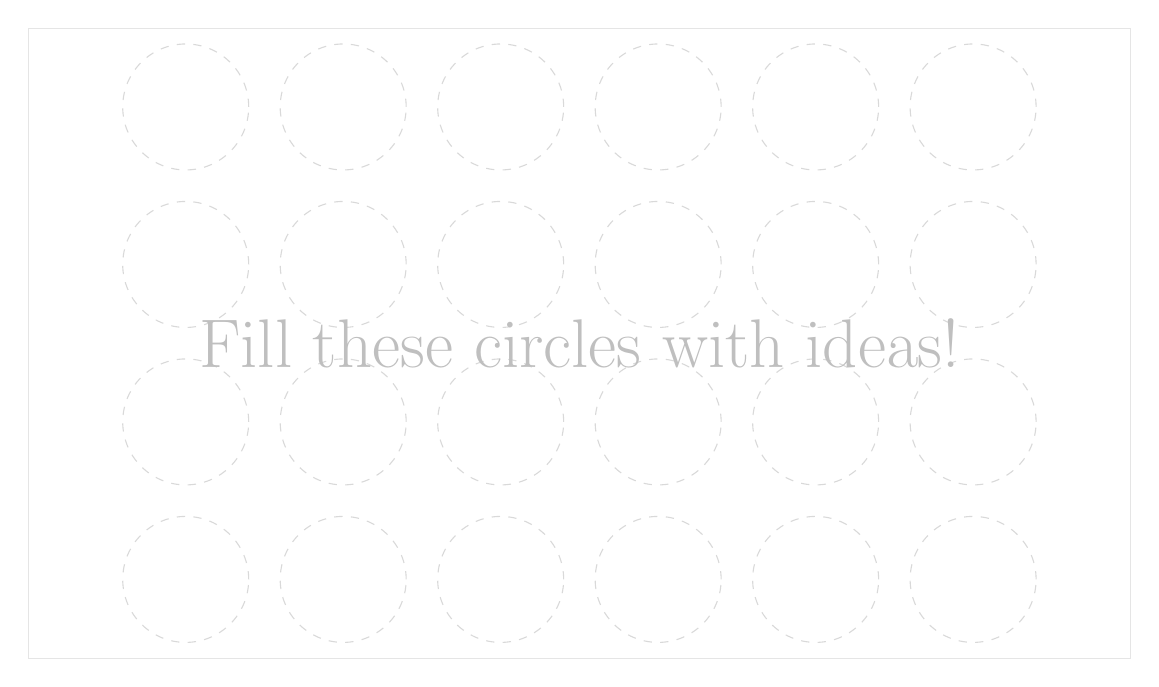
\begin{tikzpicture}
\draw[gray!20] (0,0) rectangle (14,8);
\foreach \x in {2,4,6,8,10,12} {
    \foreach \y in {1,3,5,7} {
        \draw[gray!30, dashed] (\x,\y) circle (0.8);
    }
}
\node[gray!50] at (7,4) {\Huge Fill these circles with ideas!};
\end{tikzpicture}
\end{center}

\newpage

\section*{Phase 2: Focus}

\begin{center}
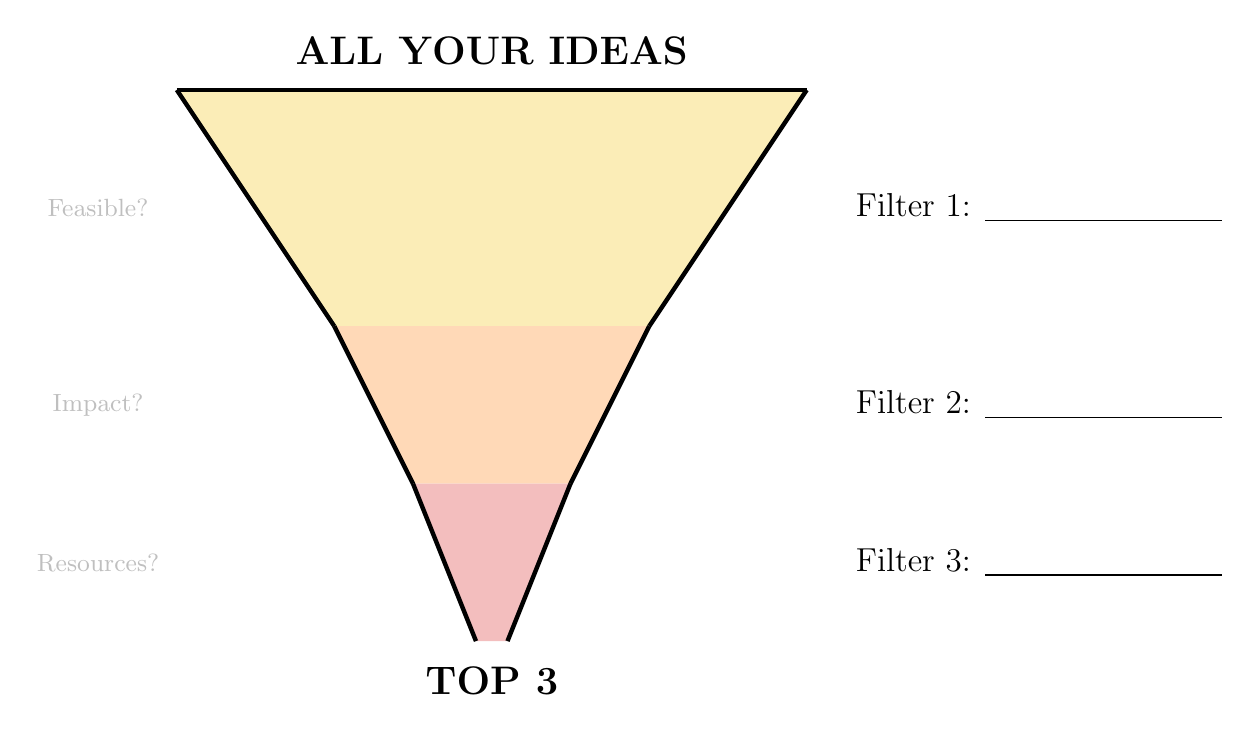
\begin{tikzpicture}[scale=1]
% Funnel shape
\fill[mlyellow!30] (2,7) -- (10,7) -- (8,4) -- (4,4) -- cycle;
\fill[mlorange!30] (4,4) -- (8,4) -- (7,2) -- (5,2) -- cycle;
\fill[mlred!30] (5,2) -- (7,2) -- (6.2,0) -- (5.8,0) -- cycle;

\draw[ultra thick] (2,7) -- (10,7);
\draw[ultra thick] (2,7) -- (4,4);
\draw[ultra thick] (10,7) -- (8,4);
\draw[ultra thick] (4,4) -- (5,2);
\draw[ultra thick] (8,4) -- (7,2);
\draw[ultra thick] (5,2) -- (5.8,0);
\draw[ultra thick] (7,2) -- (6.2,0);

% Labels
\node at (6,7.5) {\Large\textbf{ALL YOUR IDEAS}};
\node[right] at (10.5,5.5) {\large Filter 1: \underline{\hspace{3cm}}};
\node[right] at (10.5,3) {\large Filter 2: \underline{\hspace{3cm}}};
\node[right] at (10.5,1) {\large Filter 3: \underline{\hspace{3cm}}};

\node at (6,-0.5) {\Large\textbf{TOP 3}};

% Example filters (grayed out)
\node[gray!50, font=\small] at (1,5.5) {Feasible?};
\node[gray!50, font=\small] at (1,3) {Impact?};
\node[gray!50, font=\small] at (1,1) {Resources?};
\end{tikzpicture}
\end{center}

\vspace{2em}

\section*{Your Final 3}

\begin{center}
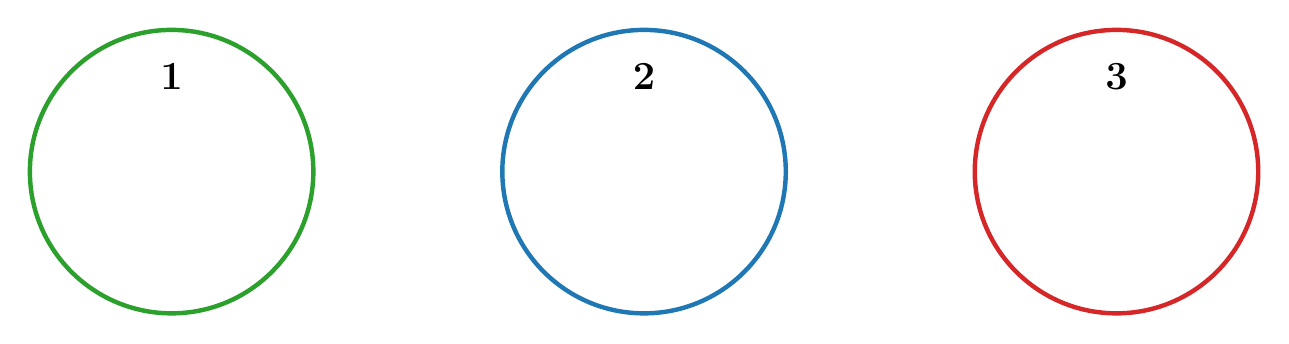
\begin{tikzpicture}[scale=1.2]
\draw[ultra thick, mlgreen] (0,0) circle (1.5);
\node at (0,1) {\Large\textbf{1}};

\draw[ultra thick, mlblue] (5,0) circle (1.5);
\node at (5,1) {\Large\textbf{2}};

\draw[ultra thick, mlred] (10,0) circle (1.5);
\node at (10,1) {\Large\textbf{3}};
\end{tikzpicture}
\end{center}

\vspace{3em}

\section*{The Scale Problem}

\begin{center}
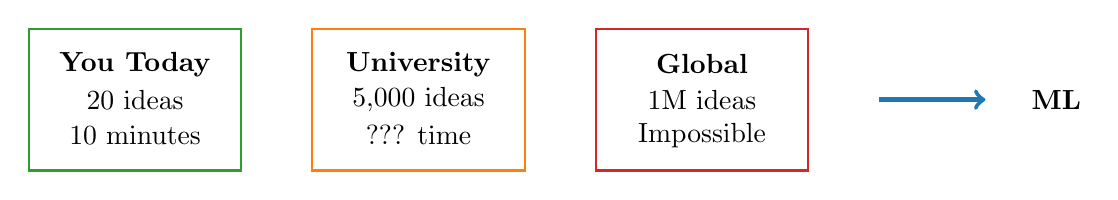
\begin{tikzpicture}[scale=0.9]
% You
\draw[thick, mlgreen] (0,0) rectangle (3,2);
\node at (1.5,1.5) {\textbf{You Today}};
\node at (1.5,1) {20 ideas};
\node at (1.5,0.5) {10 minutes};

% University
\draw[thick, mlorange] (4,0) rectangle (7,2);
\node at (5.5,1.5) {\textbf{University}};
\node at (5.5,1) {5,000 ideas};
\node at (5.5,0.5) {??? time};

% Global
\draw[thick, mlred] (8,0) rectangle (11,2);
\node at (9.5,1.5) {\textbf{Global}};
\node at (9.5,1) {1M ideas};
\node at (9.5,0.5) {Impossible};

% Arrow
\draw[->, ultra thick, mlblue] (12,1) -- (13.5,1);
\node at (14.5,1) {\textbf{ML}};
\end{tikzpicture}
\end{center}

\vspace{2em}

\begin{tcolorbox}[colback=mlblue!10, colframe=mlblue!50]
\centering\large
\textbf{Next Class:} How ML handles millions of ideas in seconds
\end{tcolorbox}

\end{document}